\documentclass{article}
\usepackage[utf8]{inputenc}
\usepackage[english]{babel}
\usepackage{graphicx}
\usepackage{multicol}
\usepackage[pdftex,
            pdfauthor={Justin Meiners},
            pdftitle={Live Hmong},
            pdfsubject={Hmong, Hmoob Language},
            pdfkeywords={Hmong, Hmoob, words, vocabulary, dictionary, learning, language, culture, resources, education, school.}]{hyperref}

\title{Live Hmong}
\author{Justin Meiners and Ku Moua}
\date{December 2014}

\begin{document}
\begin{titlepage}

\null\hfill\begin{tabular}[t]{l@{}}
  \textbf{v1.1}
\end{tabular}

\begin{center}

\setlength\fboxsep{0pt}
\setlength\fboxrule{0.0pt}
\fbox{
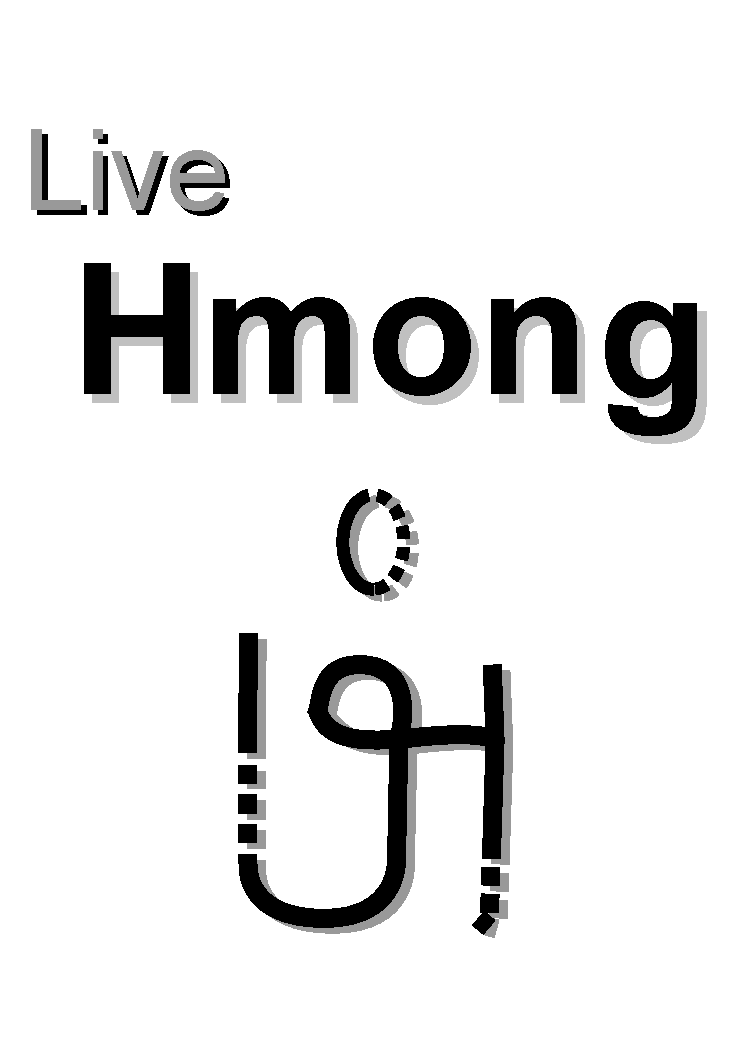
\includegraphics[scale=0.85]{cover}}

 \textbf{Live Hmong} \\
\large A book of basic Hmong words. \\
(ib phau ntawv txog lus Hmoob.) \\
~ \\
Justin Meiners and Ku Moua \\
December 2014

\end{center}

\end{titlepage}

\section*{\centering{Introduction}}
Live Hmong is a small collection of basic vocabulary words for beginners.
Most Hmong vocabulary resources are organized like dictionaries, and try to cover a wide list of words overwhelming, and unnecessary for most beginners.
Live Hmong is unique in that organizes words based on life context to give beginners a grasp of everyday language.
 It also focuses on mostly single symbol words, which provide intuition and foundation for understanding compound words.

I created this guide, with help from my teacher Ku Moua, to help me while I was studying Hmong.
I am by no means a language expert and the book likely contains mistakes. If you have any suggestions or contributions feel free to contact me at justin.meiners@gmail.com.

\hfill - Justin Meiners

\clearpage


\begin{multicols}{2}
[
\section*{\centering{Basics}}
]

\begin{tabular}{l r}
\textbf{Colors} \\
~\\

dawb {\em (xim)} &white\\
daj {\em (xim)} &yellow\\
dub {\em (xim)} &black\\
nstuav {\em (xim)} &green\\
kas fes {\em (xim)} &brown\\
liab {\em (xim)} &red\\
xiav {\em (xim)} &blue\\
paj yeeb {\em (xim)} &purple\\
txaij {\em (xim)} &striped\\
txho tshuav {\em (xim)} &gray\\
xoob {\em (xim)} &orange\\
\end{tabular}

\begin{tabular}{l r}
\textbf{Numbers} \\
~\\
ib &1\\
ob &2\\
peb &3\\
plaub &4\\
tsib &5\\
rau &6\\
xya &7\\
yi &8\\
cuaj &9\\
kaum &10\\
\end{tabular}
\end{multicols}

\begin{tabular}{l r}
\textbf{Classifiers} \\
~\\
lub &round, large, buildings\\
tus &people, animals, long, straight, systems\\
leej &important people\\
phau &books\\
daim &flat objects\\
txoj &abstract, long flexible\\
zaj &paragraphs, speeches\\
lo &single words\\
tsob &single words\\
rab &tools used with hands\\
nkawm &pairs\\
pob &packets\\
pluas &meals\\
yav &time of day\\
pawg &groups, herds\\
cov, tej &pluralizers\\

\end{tabular}

\clearpage


\begin{multicols}{2}
[
\section*{\centering{People, Friends, and Family}}
]

\begin{tabular}{l r}
\textbf{Nouns} \\
~\\
neeg {\em (tus)} &person\\
kws {\em (tus)} &skilled expert\\
laib {\em (tus)} &punk\\
neej {\em (lub)} &life\\
niam {\em (tus)} &mother\\
ntxhais {\em (tus)} &daughter\\
npe {\em (lub)} &name\\
pog {\em (tus)} &grandmother\\
phooj ywg {\em (tus)} &friend\\
tub {\em (tus)} &son\\
txiv &father\\
txiv {\em (tus)} &husband\\
yawg {\em (tus)} &grandfather\\
\end{tabular}

\begin{tabular}{l r}
\textbf{Verbs} \\
~\\
haum &get along/fit\\
hlub &love\\
hu &call\\
khav &brag\\
laum &tickle\\
luag &laugh\\
mloog &listen\\
nco &miss\\
noog &ask\\
nwj &kiss\\
ntsib &meet\\
ntxhi &whisper\\
nyiam &like\\
pab &help\\
quaj &cry\\
qawm &hug\\
teb &answer\\
xav &want\\
\end{tabular}

\end{multicols}

\clearpage

\begin{multicols}{2}
[
\section*{\centering{Clothing}}
]

\begin{tabular}{l r}
\textbf{Nouns} \\
~\\
tiab {\em (daim)} &shirt\\
tiab {\em (lub)} &dress\\
kaus mom {\em (lub)} &hat\\
khau {\em (nkawm, lub)} &shoes\\
khia mis {\em (lub)} &bra\\
hnab {\em (lub)} &bag\\
moo {\em (lub)} &watch\\
nplhaib {\em (lub)} &ring\\
saw {\em (txoj)} &necklace\\
thoom thaub &socks\\
tsho {\em (lub)} &shirt\\
ris {\em (lub)} &pants\\
\end{tabular}

\begin{tabular}{l r}
\textbf{Verbs} \\
~\\
hle &take off\\
hnav &put on\\
rhuav &tear\\
xaws &sew\\
\end{tabular}

\end{multicols}

\clearpage


\begin{multicols}{2}
[
\section*{\centering{Household}}
]

\begin{tabular}{l r}
\textbf{Nouns} \\
~\\
hoob {\em (lub)} &room\\
duab {\em (daim)} &picture\\
khw {\em (lub)} &store\\
khoom &stuff\\
ncej {\em (tus)} &pole/pillar\\
ntaub {\em (daim)} &cloth\\
qhov rais {\em (lub)} &window\\
qhov rooj {\em (lub)} &door\\
rooj {\em (nkawm)} &table\\
teeb {\em (lub)} &light\\
tog {\em (lub)} &chair\\
tsev {\em (lub)} &house\\
tsheb {\em (lub)} &car\\
tshuab {\em (lub)} &machine\\
txaj {\em (lub)} &bed\\
txee {\em (lub)} &cabinet\\
\end{tabular}

\begin{tabular}{l r}
\textbf{Verbs} \\
~\\
da dej &bathe\\
hau lwm &work\\
kaw &close\\
los &come (family)\\
ncaim &leave\\
nyiag &steal\\
muag &sew\\
poob &misplace/lose\\
qhib &open\\
so &rest\\
tawm &leave (command)\\
tsav &drive\\
tuaj &come\\
xauv &rent\\
xyuas &visit\\
yuav &buy\\
\end{tabular}
\end{multicols}

\clearpage

\begin{multicols}{2}
[
\section*{\centering{Kitchen}}
]

\begin{tabular}{l r}
\textbf{Nouns} \\
~\\
dej {\em (cov)} &water\\
dib {\em (lub)} &cucumber\\
diav {\em (lub)} &spoon\\
diav rawg {\em (rab)} &fork\\
dos {\em (lub)} &onion\\
fwj {\em (lub)} &bottle\\
khaub rhuab {\em (tus)} &mushroom\\
khob {\em (lub)} &cup\\
kua {\em (cov)} &liquid\\
kua txob {\em (lub)} &pepper\\
lauj kaub {\em (lub)} &pot\\
mij {\em (lub)} &noodles\\
mov {\em (cov, pob)} &rice\\
phaj {\em (lub)} &plate\\
nqaij {\em (daim)} &meat\\
qe {\em (lub)} &egg\\
riam {\em (rab)} &knife\\
rawg tais {\em (rab)} &chopstick\\
tais {\em (lub)} &bowl\\
tshuaj {\em (pob)} &medicine\\
txiv {\em (lub)} &fruit\\
yias {\em (pob)} &frying pan\\
zaub {\em (cov)} &vegetables\\
\end{tabular}

\begin{tabular}{l r}
\textbf{Verbs} \\
~\\
haus &drink\\
huv &clean/neat\\
noj &eat\\
nqos &swallow\\
ntxais &suck\\
ntxuav &wash\\
qhwv &wrap\\
saj &taste\\
sim &try\\
tawv &peel\\
tseg &spare\\
tsw &smell\\
tos &wait\\
zom &chew\\

\end{tabular}
\end{multicols}

\clearpage

\begin{multicols}{2}
[
\section*{\centering{Outdoors}}
]

\begin{tabular}{l r}
\textbf{Nouns} \\
~\\
av {\em (daim)} &dirt/ground\\
choj {\em (lub)} &bridge\\
hmab {\em (tsob)} &vine\\
hnub {\em (lub)} &sun\\
hli {\em (lub)} &moon\\
kev {\em (txoj)} &path\\
ncaws pob &soccer\\
nkoj {\em (lub)} &boat\\
nroj {\em (tsob)} &weed\\
ntaus pob &volley ball\\
ntoo {\em (lub)} &sky\\
nyav {\em (tus)} &valley\\
nyom {\em (cov)} &grass\\
paj {\em (lub, tsob)} &plant/flower\\
pas {\em (tus)} &stick\\
pob {\em (lub)} &ball\\
roob {\em (lub)} &mountain\\
suab {\em (tsob)} &bush\\
teb {\em (daim)} &farm\\
tuj lub {\em (lub)} &tops (game)\\
tsua {\em (lub)} &cave\\
vaj {\em (lub)} &garden\\
xyoob {\em (tsob)} &bamboo\\
zeb {\em (lub)} &rock\\
\end{tabular}

\begin{tabular}{l r}
\textbf{Verbs} \\
~\\
khawb &dig\\
nce &climb\\
ncig &explore\\
nkaum &hide\\
ntab &float\\
si &play\\

\end{tabular}
\end{multicols}

\clearpage

\begin{multicols}{2}
[
\section*{\centering{Animals}}
]

\begin{tabular}{l r}
\textbf{Nouns} \\
~\\
dais {\em (tus)} &bear\\
dev {\em (tus)} &dog\\
hma {\em (tus)} &wolf\\
kab {\em (tus)} &beetle\\
kheb {\em (luv)} &alligator\\
lom {\em (cov)} &poison\\
miv {\em (tus)} &cat\\
muv {\em (tus)} &bee\\
nas {\em (tus)} &rodent\\
nees {\em (tus)} &horse\\
noog {\em (tus)} &bird\\
npua {\em (tus)} &pig\\
nquab {\em (lub)} &dove/quail\\
ntses {\em (lub)} &fish\\
ntxhw {\em (tus)} &elephant\\
nyuj {\em (tus)} &cow\\
qav {\em (tus)} &frog\\
qaib {\em (tus)} &chicken\\
tw {\em (tus)} &tail\\
tsiaj lub {\em (tus)} &animal\\
tsov {\em (tus)} &tiger\\
vaub ki {\em (tus)} &turtle\\
yaj {\em (tus)} &sheep\\
zaj {\em (tus)} &dragon\\
\end{tabular}

\begin{tabular}{l r}
\textbf{Verbs} \\
~\\
caij &ride\\
coj &guide/lead\\
cuab &trap\\
hem &scare\\
plev &string\\
qw &scream/shout\\
tom &bite\\
tua &kill\\
tuag &die (less formal)\\
ya &fly\\
zov &care/guard\\
\end{tabular}
\end{multicols}

\clearpage

\begin{multicols}{2}
[
\section*{\centering{Body}}
]

\begin{tabular}{l r}
\textbf{Nouns} \\
~\\
caj dab {\em (lub)} &neck\\
caj npab {\em (txhais)} &arm\\
ceg {\em (txhais)} &leg\\
di ncauj {\em (daim)} &lip\\
hauv caug {\em (lub)} &knee\\
hlwb {\em (lub)} &brain\\
hniav {\em (cov, tus)} &teeth\\
ko taw {\em (txhais)} &foot\\
luj tshib {\em (lub)} &elbow\\
nplaig {\em (tus)} &tongue\\
nrab qaum {\em (lub)} &back\\
ntsej muag {\em (lub)} &face\\
ntshav {\em (cov)} &blood\\
ntiv taw {\em (cov, tus)} &toes\\
ntiv tes {\em (cov, tus)} &fingers\\
ntsws {\em (lub)} &lungs\\
mob {\em (txoj)} &ache/pain\\
plab {\em (lub)} &stomach\\
plaub {\em (cov, txoj)} &hair\\
plawv {\em (lub)} &heart\\
pob nsteg {\em (lub)} &ear\\
pob tw {\em (lub)} &butt\\
pob txha {\em (tus)} &bone\\
qhov muag {\em (lub)} &eye\\
qhov ncauj {\em (lub)} &mouth\\
siab {\em (lub)} &liver\\
taub hau {\em (lub)} &head\\
tes {\em (txhais)} &hand\\
zog {\em (lub)} &energy\\

\end{tabular}

\begin{tabular}{l r}
\textbf{Verbs} \\
~\\
hais &say\\
hnov &hear\\
ev &carry\\
khiav &run\\
kov &feel (touch)\\
muaj &have\\
mus &go\\
ncaws &kick\\
nkag &crawl\\
plhaw/dhia &hop/jump\\
pom &see\\
pw &lay\\
pov &throw\\
qw &yell\\
rho &pull\\
saib &look/observe\\
sawv &stand\\
thawb &push\\
tso &drop\\
txav &move\\
\end{tabular}

\end{multicols}

\clearpage

\begin{multicols}{2}
[
\section*{\centering{Tools and Weapons}}
]

\begin{tabular}{l r}
\textbf{Nouns} \\
~\\
ciaj {\em (rab)} &pliers\\
duav {\em (rab)} &shovel\\
hlau {\em (txoj, daim)} &metal\\
hlau {\em (rab)} &hoe\\
hlua {\em (txoj)} &rope\\
hmuv {\em (rab)} &spear\\
ntaj {\em (rab)} &sword\\
ntaiv {\em (tus)} &ladder\\
ruaj {\em (rab)} &hammer\\
thoob {\em (lub)} &bucket\\
\end{tabular}

\begin{tabular}{l r}
\textbf{Verbs} \\
~\\
dam &break in two\\
hno &insert/puncture\\
kho &fix\\
koom &join\\
nkaug &stab\\
ntaus &hit/strike\\
ntsuas &mesure\\
puas &break (machinery)\\
phob &use wastefully\\
quav &separate/divide\\
siv &use\\
tawg &explode/burst\\
tu &break (tension)\\
txiav &cut/clib\\
\end{tabular}
\end{multicols}

\clearpage

\begin{multicols}{2}
[
\section*{\centering{Literature}}
]

\begin{tabular}{l r}
\textbf{Nouns} \\
~\\
dab neeb {\em (txoj)} &story\\
dab {\em (tus)} &monster\\
kev {\em (txoj)} &way of\\
lus {\em (lo, cov)} &word\\
npiv {\em (tus)} &pen\\
ntawv {\em (phau)} &book\\
moo {\em (txoj)} &news/report\\
qhov {\em (lub)} &hole/thing\\
tshooj {\em (tus)} &chapter/section\\
yeem {\em (txoj)} &symbol\\
xaum {\em (tus)} &writing utensil\\
zos {\em (lub)} &village\\
\end{tabular}

\begin{tabular}{l r}
\textbf{Verbs} \\
~\\
kawm &study/learn\\
kos &mark/engrave\\
nyeeg &read\\
paub &know\\
piav &explain\\
qhia &teach/tell\\
qaug &copy\\
sau &write\\
to taub &understand\\
txhais &translate\\
\end{tabular}
\end{multicols}

\clearpage

\begin{multicols}{2}
[
\section*{\centering{Spritual}}
]

\begin{tabular}{l r}
\textbf{Nouns} \\
~\\
plig {\em (tus)} &spirit\\
hmoov {\em (txoj)} &luck\\
mlom {\em (lub)} &idol/sculpture\\
neeb {\em (tus)} &shaman\\
tshawj {\em (lub)} &church\\
Vajtswv {\em (tus)} &god\\
\end{tabular}

\begin{tabular}{l r}
\textbf{Verbs} \\
~\\
hloov &change/evolve\\
ntseeg &believe\\
tsib &command\\
\end{tabular}
\end{multicols}

\clearpage

\begin{multicols}{2}
[
\section*{\centering{Unsorted Words}}
]

\begin{tabular}{l r}
\textbf{Nouns} \\
~\\

\end{tabular}

\begin{tabular}{l r}
\textbf{Verbs} \\
~\\
coj &bring\\
dag &lie\\
kiv &spin\\
kawg &end\\
npuaj &slap\\
nres &stop\\
ntob &hit\\
peg &beat/hit\\
pib &begin\\
poob &fall\\
rhuav &take down\\
xaiv &choose\\
\end{tabular}
\end{multicols}

\clearpage

\begin{multicols}{2}
[
\section*{\centering{Description}}
]

\begin{tabular}{l r}
\textbf{Adjectives} \\
~\\
ceev &fast\\
qeeb &slow\\
loj &big\\
me &small\\
zoo &good\\
phem &bad\\
rog &fat\\
yuag &skinny\\
ntse &smart\\
ruam &dumb\\
siab &tall\\
luv &short\\
sib &light\\
hnyav &heavy\\
ntiav &shallow\\
tob &deep\\
nyuaj &difficult\\
yooj yim &easy\\
kim &expensive\\
pheej yig &cheap\\
tuab &thick\\
nyias &thin\\
txawv &different\\
tseeb &true\\
kawg &extremely\\
kawg nkaus &incredibly\\
tsis tsua &not really\\
\end{tabular}

\begin{tabular}{l r}
\textbf{Prepositions} \\
~\\
dhau &through\\
hauv &in\\
hauv qab &under/beneath\\
ncig &around\\
nram &downhill\\
nraum &outside\\
ntawm &of\\
ntawd &that/there\\
pem &up hill\\
qab &below\\
saum &above/on\\
tim &over there\\
tom &there (near)\\
tom qab &behind\\
\end{tabular}


\end{multicols}

\end{document}
